
\section{Sensors} \label{sensors}
%\todo[inline]{Add more sensors: Infrared, Thermal, other depth sensors - evaluate them the same way as the others}
\todo[inline]{Relate to scientific work}
In order to drive on the road safely, the driver needs to have perfect awareness of what is happening around the vehicle to keep the car driving in the lane or avoid any dangerous situations. Therefore, when taking the human driver out of the picture and making the vehicle autonomous, engineers have to design a system, that will take the roles of everything the driver was responsible for. In this case, the car has to be equipped with sensors which will provide an onboard computer with all the necessary data required to drive the car safely on public roads. There are currently three types of sensors used in either semi or fully autonomous cars. These are cameras, lidar and radar which all work together to achieve a better understanding of what is happening in all directions around the car. 

\subsection{RGB Cameras}  
RGB cameras in autonomous cars serve one very important role which is very naturally done by human drivers. That is the perception of the surrounding environment which encompasses object detection and classification as well as determining distances between them and the car. 
Under the category of object detection/classification lies the understanding of the traffic, based on road signs and lights, detection of other traffic participants and absolutely anything that humans naturally use as clues to safely execute the drive between two points. 
\subsection*{Advantages}
\begin{itemize}
  \item Very high resolution and framerate especially beneficial for object classification
  \item Multiple cameras working together can measure distance to obstacles
\end{itemize}
\subsection*{Disadvantages}
  \begin{itemize}
  \item Affected greatly by light levels (solution is to include night vision camera as well)
  \item Bad weather affects performance negatively
\end{itemize} \cite{LidarRad25:online}

 
   \begin{figure}[H]
\centering
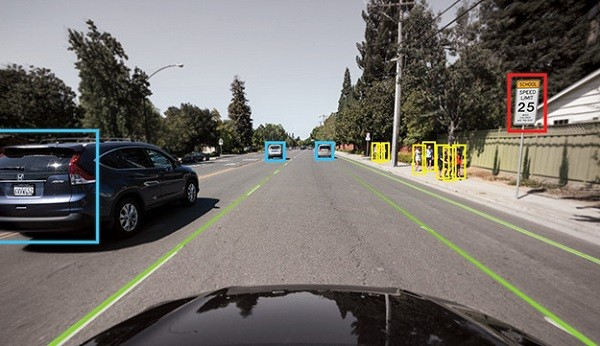
\includegraphics[width=\textwidth]{Figures/ConAnalysis/General/camera.jpg}
\caption{Object classification using cameras\cite{nvidiadr29:online}}
\end{figure}
 
\subsection{Radar}
Radar technology uses radio waves to determine the position and velocity of all the obstacles relative to the car. There are two types of radar which are used in autonomous cars - short and long range, working from a few centimetres to hundreds of meters. The primary function of radar technology in an autonomous car is to monitor traffic around the vehicle. The most common uses for this technology are to help the car stay within safe distance when following another car, help with parking and emergency braking. \cite{Autonomo37:online}

\subsection*{Advantages}
\begin{itemize}
  \item Unaffected by light levels
  \item Matured technology in automotive industry
  \item Determines not only distance to the object but also its velocity
\end{itemize}
\subsection*{Disadvantages}
\begin{itemize}
  \item Resolution not high enough for object classification
  \item Shorter range radar has problems differentiating between multiple objects
\end{itemize}
 \cite{LidarRad25:online}
 
  \begin{figure}[H]
\centering
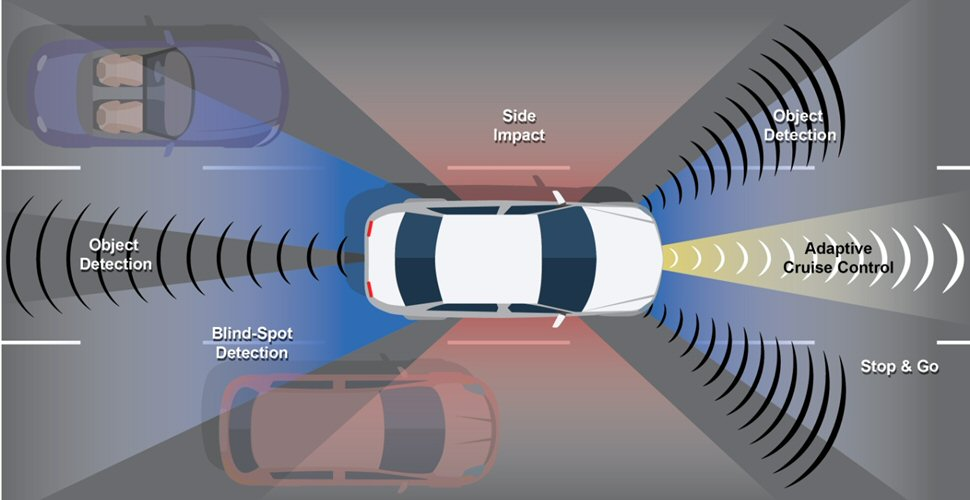
\includegraphics[width=\textwidth]{Figures/ConAnalysis/General/radar.jpg}
\caption{This figure shows what is radar used for in autonomous cars\cite{3m321F1j31:online}}
\end{figure}
\subsection{Lidar}
Lidar technology is remarkably similar to the Radar's. The difference is that it uses infrared lasers instead of radio waves. The utility it provides to the car is similar to what the radar has to offer. It can also measure the distance to the objects around the car and their velocity, but on top of that, it can create a 3D map of these objects. This helps greatly in the classification process and allows the car to make more informed decisions.\cite{Autonomo37:online}

\subsection*{Advantages}
\begin{itemize}
  \item Creates a 3D representation of the real world 360° around the car (depending on the lidar type)
  \item Unaffected by light levels
  \item Better range and distance estimation compared to stereo cameras
\end{itemize}
\subsection*{Disadvantages}
\begin{itemize}
  \item Unable to classify obstacles based on their appearance (e.g. road signs), only their shape
  \item Expensive technology 
  \item Threat of hurting the eyesight of pedestrians
\end{itemize}
 \cite{LidarRad25:online}
 
 \begin{figure}[H]
\centering
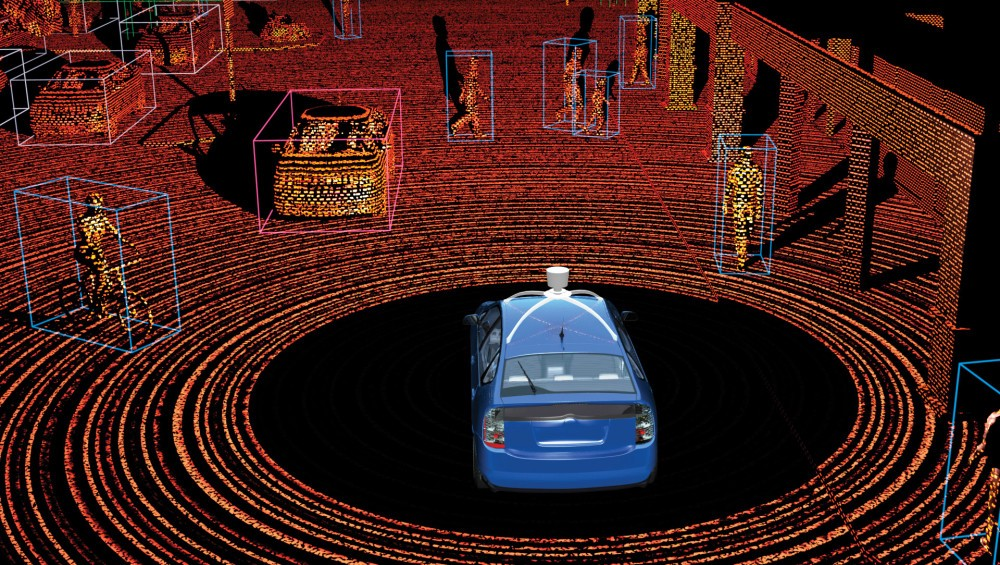
\includegraphics[width=\textwidth]{Figures/ConAnalysis/General/Lidar.jpeg}
\caption{This figure shows what car perceives using Lidar\cite{1vrB0Jrb84:online}}
\end{figure}
 
 \color{blue}

\subsection{Thermal imaging camera}
Unlike classic RGB camera which uses sensor that can detect visible light spectrum, this type of camera has sensor which is capable of capturing spectrum of light invisible to both classic RGB camera as well as naked eye. This type of camera is designed to detect infrared radiation which is emitted by environment, which in simple terms means detecting heat differences in objects. 

\subsection*{Advantages}
\begin{itemize}
  \item High refresh rate up to 30 fps
  \item Very long range - detection of humans up to 2.1 km and cars up to 5.3 km
  \item Works independent of lighting conditions
\end{itemize}

\subsection*{Disadvantages}
\begin{itemize}
  \item Lower resolution than RGB camera
  \item Worse performance during hot days due to measuring differences between temperatures
\end{itemize}

%https://www.flirmedia.com/MMC/CVS/Tech_Notes/TN_0002_EN.pdf
%https://www.thermalcameras.guide/how-thermal-imaging-cameras-work/

\subsection{Night vision cameras}
There are currently two types of technology which allows cameras to see in "night". Those are Nigh vision devices, further referred to as NVDs and Infra illuminated, further reffered to as I2. The difference between them is that NVDs are just taking in small amounts of visible light still present at night and magnifying it greatly and I2 need built in infrared illuminator and sensor which detects the reflected infrared light. 

\subsection*{Advantages}
\begin{itemize}
  \item Both NVDs and I2 can see in dark without needing to illuminating the scene
\end{itemize}

\subsection*{Disadvantages}
\begin{itemize}
  \item Low contrast
  \item NVDs work only in very specific light conditions, any added light source renders them useless
  \item I2 have range only as long as strong is the illuminator
\end{itemize}

%https://www.flir.com/discover/ots/thermal-vs-night-vision/
\color{black}